\documentclass{article}
\usepackage{graphicx}
\usepackage[utf8]{inputenc}
\usepackage[english]{babel}
\usepackage{listings}
\usepackage{amssymb}
\usepackage{amsmath}
\usepackage{bbold}
\usepackage{color}
\usepackage{url}
\usepackage{float}
\usepackage{epstopdf}
\setlength{\parindent}{2em}
\begin{document}
\title{Study of white dwarf stars with 4th order Runge-Kutta method}
\author{Xingze Mao}
\maketitle


\begin{center}
$\mathbf{Abstract}$
\end{center}
A code using $4^{th}$ order Runge-Kutta method is developed to study white dwarf stars. The stability of the code is studied first with different step size $h$. The dependence of the mass and radius on the central density is studied. The total kinetic and rest energy of electrons is calculated, so is the gravitational energy of the white dwarf star. Stars of elements $^{56}$Fe and $^{12}$C are calculated to study the mass-radius relation. The results are compared with the observed quantities of three dwarf stars( Sirius B, 40 Eri B and Stein 2051) and components of the three planets are determined.

\section{Introduction}
A white dwarf is what stars like the Sun become after they have exhausted their nuclear fuel. Without the energy released by the nuclear reaction, the planet will not be able to create enough outward pressure to hold itself. Under the power of gravity, everything on the planet will be pulled into the center. Heavier elements go deeper to the center and lighter nuclei remain at the surface,which gives white dwarf stars almost pure hydrogen or helium atmosphere. As gravity keeps shrinking the size of the planet, density of matter is increasing. However, this process can not keep going. Lots of electrons are squeezed together within smaller space. Density of electrons are very high.  Pauli exclusion principle does not allow two electrons in the same state. When all states are occupied by electrons, the gravity can not squeeze the planet any further. The gravity is balanced by the force of pauli exclusion principle.  Nucleons , aslo fermions, are not considered, as they have masses thousands time larger than electrons and has less kinetic energy compared to electrons. Thus we assume the outward pressure balancing the gravity mainly come from electrons. And if the star has larger mass, the schrinking process can keep going and electrons can be absorbed into protons to build nutrons, which will end up with neutron stars or black holes. This mass limit of white dwarf stars is 1.4 times the mass of the Sun($M_{\odot}$), discovered by Subrahmanyan Chandrasekhar, also known as "Charndrasekhar limit". A typical white dwarf is half as massive as the Sun, and slightly bigger than the Earth. White dwarf stars are also known to be one of the densest collections of matter, second only to neutron star. Unless it is accreting matter from a nearby star, the white dwarf cools down by emitting X-rays or extreme ultraviolet\cite{white}. This article is organized as followed: section 2 explains the theoretical background and the fourth-order Runge-Kutta method,a short introduction to code is also included in the this part; Section 3 talks about the result and explanation and followed by the conclusion in section 4.

\section{Model and method}
\subsection{Free electron gas model}
The state of the dwarf star we want to study is in both thermal and charge equilibrium. The pulling inward pressure is balanced by the pushing outward pressure of degenerate electrons. Protons' number is the same with electrons' number. As temperature of the planet is much smaller than the Fermi temperature of the electrons, we use the pressure of degenerate electrons at $T=0$ K. Electrons are assumped to be relativistic. Protons and neutrons have much lower kinetic energy and assumed to have negilible contribution to the outward pressure compared with electrons. Thus the pressure to balance the gravity is mainly set up by electrons. The kinetic energy of electrons is much larger than the repulsion between electrons or attraction from the nuclei. In other words, we treat the system as a gas of free degenerate electrons at $T=0$ moving in between a lattice of nuclei like iron\cite{computational_dwarf_star}. 
The gravitational force on every piece element with r distance away from the center of the planet is 
\begin{equation}
F_{Grav}(r) = -\frac{Gm(r)}{r^2} \rho(r),
\end{equation}
where $G$ is the gravitational constant, $\rho(r)$ is the mass density of a volume element with distance r from the center of the planet, and $m(r)$ is the total mass of the planet within radius r. And we also have the reltaion that 
\begin{equation}
m(r)=\int_{0}^{r}4\pi \rho(r')r'^2 dr'
\label{eq:m}
\end{equation}
Eq (\ref{eq:m}) can also be written in the form of differential euqtion 
\begin{equation}
\frac{dm(r)}{dr}= 4\pi r^2 \rho(r)
\end{equation}
In the equilibrium state, we have the balance between the gravitational force and the pressure generated by degenerate electron gas:
\begin{equation}
\frac{dP}{dr} = -\frac{Gm(r)}{r^2}\rho(r)
\end{equation}
As $\frac{dP}{d\rho} =(\frac{d\rho}{dr})(\frac{dP}{d\rho})$, we obtain:
\begin{equation}
\frac{d\rho}{dr} = - (\frac{dP}{d\rho})^{-1}\frac{Gm}{r^2}\rho
\label{eq:rho}
\end{equation}
So eq(\ref{eq:m}) and eq(\ref{eq:rho}) are two coupled first-order differential equation. The term $(\frac{dP}{d\rho})^{-1}$ is determined by the equation of state of the white dwarf star. With central density, we can integrate these two equations to some point R, where the density become 0. This R is the radius for the dwarf star. Also, $m=0$ at $r=0$, and the total mass of the planet is the integral of $\rho(r)$ in region $[0,R]$

\subsection{Equation of state for a white dwarf star}
In statistical physics, number of particle corresponds to the density of states in the phase space. And electrons, as femions, can have spin up and down two states, which gives us two-fold degeneracy. And in our model here, electrons are treated as a relativistic gas of fermions at $T=0$K,
\begin{equation}
n=N/V=\frac{2}{V}\int_{0}^{k_F}\frac{d\vec{r}d\vec{k}}{(2\pi)^3}=2\frac{4\pi V}{8V\pi^3} \int_{0}^{k_F}k^2dk=\frac{ k_F^3}{3\pi^2},
\label{eq:n}
\end{equation}
$k_F$ corresponds to the momentum at the Fermi energy point. Also the energy density is $\varepsilon =E/V=\frac{1}{\pi^2}\int_{0}{k_F}k^2\sqrt{(\hbar ck)^2 + m_e^2c^4}$
The integration is in the form of $\int y^2\sqrt{y^2+a^2}$ and performing the integration will give us 
\begin{equation}
 \varepsilon=n_0m_ec^2x^3 \epsilon(x),
\label{eq:energy_density}
\end{equation}
where $\epsilon(x)=\frac{3}{8x^3}\big(  x(1+2x^2)\sqrt{1+x^2} -ln(x+\sqrt{1+x^2})  \big)$ and $x=\frac{\hbar k_F}{m_e c}$
Using eq(\ref{eq:n}), we can replace the $k_F$ in the expression of $x$ by $n$, which is 
\begin{equation}
x=\frac{\hbar k_F}{m_ec} =(\frac{\hbar^3 k_F^3}{m_e^3c^3})^{1/3}=(\frac{3\pi^2n\hbar^3}{m_e^3c^3})^{1/3} =(\frac{n}{n_0})^{1/3},
\end{equation}
where $n_0=\frac{m_e^3 c^3}{3\pi^2 \hbar^3}=5.89 \times 10^{29} cm^{-3}$. As nucleon has the mass 1000 times heavier than electron, density of white dwarf star comes mainly from nucleons.  The mass density is given by
\begin{equation}
\rho = M_p n_p,
\end{equation}
where $M_p$ is the maas of proton and $n_p$ is the number of nculeons. The mass difference between protons and neutrons is neglected. The nucleon density $n_p$ is related to the electron density $n$ by $n_p=n/Y_e$, where $Y_e$ is the number of electrons per nucleon. Thus density of the planet is $\rho = \frac{M_p n}{Y_e}$. And we also have the relation $x =(\frac{n}{n_0})^{1/3} = (\frac{\rho}{\rho_0})^{1/3}$, with $\rho_0 =\frac{M_p n_o}{Y_e}= 9.79\times 10^5 Y_e^{-1}g cm^{-3}$. $Y_e$ decides what kind of element is building the planet  and the central density $\rho_c$ will affect the initial condition of the coupled differential equation and thus the radius and total mass of the planet.

Next we will find the equation for the pressure.
\begin{equation}
P=-\frac{\partial E}{\partial V} = -\frac{\partial E}{\partial x} \frac{\partial x}{\partial V},
\end{equation}
From abouve relation, we know $x\propto n^{1/3} \propto V^{-1/3}$, thus we have
\begin{equation}
\frac{\partial x}{\partial V}= - \frac{x}{3V},
\end{equation}
And aslo
\begin{equation}
\begin{aligned}
\frac{\partial E}{\partial x}& =\frac{\partial V \varepsilon}{\partial x} =\frac{V \partial \varepsilon}{\partial x}+ \frac{\varepsilon \partial V}{\partial x} \\
&=Vn_0m_e c^2 (3x^2\epsilon(x) + x^3 \frac{d \epsilon}{dx})- \frac{3V}{x}n_0m_ec^2x^3\epsilon(x) \\
&=Vn_0m_e c^2x^3 \frac{d \epsilon}{dx}.
\end{aligned}
\end{equation}
Thus
\begin{equation}
P=Vn_0m_e c^2x^3 \frac{d \epsilon}{dx} (-\frac{x}{3V}) =\frac{1}{3}n_0m_ec^2x^4\frac{d\epsilon}{dx}.
\label{eq:P}
\end{equation}
Our goal is to find $(\frac{dP}{d\rho})^{-1}$, and as $x=(\frac{\rho}{\rho_0})^{1/3}$, we can reach our goal by the following step:
\begin{equation}
\frac{dP}{d\rho} =\frac{dP}{dx}\frac{dx}{d \rho}.
\end{equation}
With eq(\ref{eq:P}), we can calculate the first derivative of $P$ with respect to $x$:
\begin{equation}
\frac{dP}{dx}=\frac{1}{3}n_0m_ec^2 \frac{dx^4 \frac{d\epsilon}{dx}}{dx}.
\end{equation}
Based on the expression of $\epsilon(x)$ below eq(\ref{eq:energy_density}), we have 
\begin{equation}
\begin{aligned}
\frac{d\epsilon}{dx}=&\frac{3}{8x^3}\big((1+6x^2)\sqrt{1+x^2} + (x+2x^3)\frac{x}{\sqrt{1+x^2}}  - \frac{1}{\sqrt{1+x^2}}\big) \\
&- \frac{9}{8x^4}\big(  (x+2x^3)\sqrt{1+x^2}  - ln(x+ \sqrt{1+x^2})   \big)  \\
=&\frac{3}{8x^3}\frac{1+7x^2 + 6x^4 +x^2 +2x^4 -1}{\sqrt{1+x^2}}  \\
& - \frac{9}{8x^4}\big(  (x+2x^3)\sqrt{1+x^2}  - ln(x+ \sqrt{1+x^2})   \big)  \\
=&\frac{3\sqrt{1+x^2}}{x} - \frac{9}{8x^4}\big(  (x+2x^3)\sqrt{1+x^2}  - ln(x+ \sqrt{1+x^2})   \big) \\
=&-\frac{3}{8}\big( (\frac{3}{x^3} -\frac{2}{x})\sqrt{1+x^2} - \frac{3}{x^4} ln(x+\sqrt{1+x^2}) \big).
\end{aligned}
\end{equation}
And then
\begin{equation}
\begin{aligned}
\frac{dx^4\frac{d\epsilon}{x}}{dx}=&\frac{d}{dx} (-\frac{3}{8}\big( (\frac{3}{x^3} -\frac{2}{x})\sqrt{1+x^2} - \frac{3}{x^4} ln(x+\sqrt{1+x^2}) \big)) x^4 \\
=& -\frac{3}{8}\big(  (3-6x^2)\sqrt{1+x^2} + \frac{3x^2-2x^4}{\sqrt{1+x^2}} -\frac{3}{\sqrt{1+x^2}}  \big)  \\
=&\frac{3x^4}{\sqrt{1+x^2}}.
\end{aligned}
\end{equation}
And also we have
\begin{equation}
\frac{dx}{d\rho}= \frac{1}{3} \rho^{-2/3} \rho_0^{-1/3 }=\frac{1}{3\rho_0 x^2}.
\end{equation}
So we have 
\begin{equation}
\frac{dP}{d\rho} =\frac{1}{3}n_0m_ec^2  \frac{3x^4}{\sqrt{1+x^2}} \frac{1}{3\rho_0 x^2} =m_ec^2 \frac{n_0}{\rho_0} \frac{x^2}{\sqrt{1+x^2}} = Y_e \frac{m_ec^2}{M_p} \gamma(x),
\end{equation}
where $\gamma(x)= \frac{x^2}{3\sqrt{1+x^2}}$. Plugging this term back to the eq(\ref{eq:rho}), we then have all the terms to solve the two coupled equations for the white dwarf stars.

\begin{equation}
\begin{aligned}
&\frac{d\rho}{dr} = -   \frac{M_p}{Y_e \gamma(x) m_e c^2}  \frac{Gm}{r^2}\rho  \\
&\frac{dm}{dr} = 4\pi r^2 \rho(r).
\end{aligned}
\end{equation}

\subsection{Dimensionalless form of the differential equations}
In the situation when we deal with the white dwarf stars, quantities with different order shows up in the same equations, if we just go ahead and do the calculation blindly by plugging all the quantities with their values, we may encounter large error in our final resutl. For example, mass of the sun is approximately $2\times 10^{30} $kg and mass of the electron is $9\times 10^{-31}$kg. In the same equation, mass of the electron will be treated as 0 by the computer. Mistakes will be made in this way. To avoid this problem, we use dimensionless form of the differential equation.

We introduce three dimensionless quantity: dimensionless radius $\bar{r} = r/R_0$, dimensionless density $\bar{\rho} = \rho/\rho_0$ and dimensionless mass $\bar{m} = m/M_0$.  Plugging these quantities into the differential equation for mass, we have
\begin{equation}
\frac{dm}{dr}=4\pi r^2 \rho(r)  \rightarrow \frac{dM_0 \bar{m}}{dR_0 \bar{r}}= 4\pi R_0^2 \bar{r}^2 \rho_0 \bar{\rho},
\end{equation}
Moving all the coefficients to the right side of the differential equation, we have 
\begin{equation}
\frac{d\bar{m}}{d\bar{r}}=4\pi R_0^3 \bar{r}^2  \rho_0  \bar{\rho}/M_0.
\end{equation}
The coefficient of this equation should be dimensionless because all other terms in the equations are dimensionless. For simplicity we assume this coefficient to be 1. Then we have $M_0 = 4\pi R_0^3 \rho_0$. 
In the same way, we have a similar expression for the differential equation for the density $\rho$,
\begin{equation}
\frac{d\rho_0 \bar{\rho}}{dR_0 \bar{r}} = -\big(   \frac{GM_0M_p}{Y_e m_e  c^2} \big)  \frac{\bar{m}}{\gamma R_0^2 \bar{r}^2} \rho_0 \bar{\rho},
\end{equation}
and then we have 
\begin{equation}
\frac{d \bar{\rho}}{d \bar{r}}= - -\big(   \frac{GM_0M_p}{Y_e m_e  c^2} \big) \frac{1}{R_0} \frac{\bar{m} \bar{\bar{\rho}}}{\gamma \bar{r}^2},
\end{equation}
so $R_0 =\frac{GM_0M_p}{Y_e m_e  c^2} $. Together with the relation $M_0 = 4\pi R_0^3 \rho_0$, we have $R_0=\big(\frac{Y_e m_e C^2}{4\pi \rho_0 G M_p} \big)^{1/2} = 7.72 \times 10^8 Y_e$cm and $M_0 =5.67 \times 10^{33} Y_e^2$g. After using the dimensionless parameter, our final equations become
\begin{equation}
\frac{d\bar{\rho}}{d\bar{r}} = - \frac{\bar{m}}{\gamma \bar{r}^2} \bar{\rho},    \qquad      \frac{d \bar{m}}{d \bar{r}}=\bar{r}^2 \bar{\rho}.
\end{equation}

\subsection{Runge-Kutta method}
For normal differential equation in the form of $\frac{dy}{dx}= f(x)$, we can use many different ways like Euler method, Verlet method and so on, to solve them. But if the function $f$ also depends on
 $y$, like $\frac{dy}{dx}= f(x,y)$, we will need a different method to get it work. Runge-Kutta(RK) methods can be a good choice here. Runge-Kutta methods are also based on Taylor expansion formulae, but intermediate steps are added to update the new dependent variables.
Here we consider the 2nd order Runge-Kutta method to solve $\frac{dy}{dx}= f(x,y)$ first:
\begin{equation}
y_{i+1} =y_i + \int_{x_i}^{x_{i+1}} f(x,y)dx.
\end{equation}  
If we expand both $y_{i+1}$ and $y_i$ at point $y_{i+1/2}$,we can get the following relation:
\begin{equation}
y_{i+1} =y_i + hf(x_{i+1/2}, y_{i+1/2}) +O(h^3).
\end{equation}
The value of $y_{i+1/2}$ is obtained by Euler's method
\begin{equation}
y_{i+1/2}= y_i + \frac{h}{2}\frac{dy}{dx}= y_i+ \frac{h}{2}f(x_i,y_i).
\end{equation}
Then we get the second-order Runge-Kutta method:
\begin{equation}
k_1= h f(x_i,y_i)
k_2 = h f(x_{i+1/2},y_i+k_1/2)
y_{i+1} = y_i + k_2 + O(h^3).
\end{equation}

And for the fourth-order Runge-Kutta method, we have\cite{Computational}
\begin{equation}
\begin{aligned}
\quad k_1 =hf(x_i,y_i) \qquad k_2=hf(x_i+h/2,y_i+k_1/2)\\
k_3=hf(x_i+h/2,y_i + k_2/2) \qquad k_4=hf(x_i+h, y_i+k_3)\\
y_{i+1} = y_i +\frac{1}{6}(k_1+2k_2+2k_3+k_4).
\end{aligned}
\end{equation}

\subsection{Short intro to the code }
The code is divided into mainly two parts: one part to update the density and mass using 4th-order Runge-Kutta method, which is in file "ode\_method.cpp", the other part is calculation on energies based on the updated density and mass in the main function file "main.cpp".

The following part is the main function part. Loop stops when $\rho<10^{-6}$. Within each loop, a function is called first to update mass and density for the next point, which is followed by two functions, one calculating the total kinetic and rest energy of electrons and the other one calculating the gravitational energy.
\begin{lstlisting}[frame=single]
while(rho_old>1.0e-6)
{//update m  and rho by Runge-Kutta 4th order method;
	dwarf_star(r,h,rho_old,m_old, rho_new, m_new);
	//update parameters	
	rho_old=rho_new;
	m_old=m_new;
	r+=h;
	//calculate kinetic energy
	double x=pow(rho_new,1.0/3.0);
	rest_kinetic_e+=dwarf_star.epsilon_f(x)*r*r*h;
	//calculate the gravitational energy
	grav_e+= rho_new*m_new*r*h;
	}
}
\end{lstlisting}

The code below shows how the 4th-order Runge-Kutta method is applied to update the mass and density
\begin{lstlisting}[frame=single]
void RK4_class::operator()(const double &r,const double &h, 
const double &rho_old, const double &m_old,double &rho_new,
double &m_new)
{
	//first point
  double gamma=gamma_f(rho_old);
  double k1_m = h* m_function( rho_old, r);
  double k1_rho=h*rho_function( -m_old/gamma,r,rho_old);

  double m1 = m_old+ k1_m/2.0;
  double rho1 = rho_old + k1_rho/2.0;
  //first mid-point
  gamma=gamma_f(rho1);
  double k2_m = h* m_function(rho1,r+0.5*h);
  double k2_rho =h*rho_function(-m1/gamma,r+0.5*h,rho1);

  double m2 = m_old+ k2_m/2.0;
  double rho2 = rho_old+ k2_rho/2.0;
  //second mid-point
  gamma=gamma_f(rho2);
  double k3_m = h*m_function(rho2, r+0.5*h);
  double k3_rho=h*rho_function(-m2/gamma,r+0.5*h,rho2);

  double m3 = m_old+ k3_m;
  double rho3 = rho_old+ k3_rho;
  //last point
  gamma=gamma_f(rho3);
  double k4_m = h*m_function(rho3, r+h);
  double k4_rho = h*rho_function(-m3/gamma, r+h, rho3);
  m_new=m_old +(k1_m + 2.0*k2_m + 2.0*k3_m + k4_m)/6.0;
  rho_new=rho_old+(k1_rho+2.0*(k2_rho+k3_rho)+k4_rho)/6;
}
\end{lstlisting}

\section{Results and discussion}
\subsection{dependence of mass and radius on central density}
\begin{table}[H]
\centering
\begin{tabular}{|c|c|c|c|c|}
\hline
$\rho_c /\rho_0$& $10^{-1}$& $10^{0}$ & $10^{1}$  & $10^{2}$  \\
\hline
radius /$R_{\odot}$& 0.0417599&  0.0277496&   0.0176797&  0.0105964\\
\hline
mass /$M_{\odot}$& 0.797289&  2.0146&  3.69836&  4.94496\\
\hline
$\rho_c /\rho_0$&  $10^{3}$  & $10^{4}$  & $10^{5}$  & $10^{6}$ \\
\hline
radius /$R_{\odot}$& 0.00592667& 0.00310167& 0.00154136 & 0.000741232\\
\hline
mass /$M_{\odot}$&5.50714&  5.68876&  5.73625 &  5.74732\\
\hline
\end{tabular}
\caption{Dependence of mass and radius on central density}
\label{tab:rho_dependence}
\end{table}
We have two parameters to control the results of the coupled differential equations. $Y_e$ controls the component element of the planet amd central density $\rho_c$ sets up the initial condition for our calculation. With different central density, we will end up with different radius and mass. Table(\ref{tab:rho_dependence}) shows us the radius and mass of our planets with different central density $\rho_c$. In these calculations, $Y_e=1$ is used and the step size $h$ is set to be $10^{-7}$. Mass and radius are in the unit of mass of sun $M_{\odot}= 1.99\times 10^{33}$g and radius of Sun $R_{\odot}=6.95 \times 10^{10}$ cm respectively.  Density is in the unit of $\rho_{0}=9.79 \times 10^5 Y_e^{-1}$gcm$^{-3}$. The results are also shown in fig (\ref{fig:rho_dependence}) and it's more clear that with larger central density, the size of the planet gets smaller and the mass of the planet gets bigger. It makes sense because larger central density has larger attractive gravitational force, which pulls everything into the center and thus gives us smaller size of the planet. However, since the density is much bigger, the overall mass of mass is increasing with central density.


\begin{figure}[H]
\centering
\includegraphics[width=8cm,angle=270]{m_r_rho.eps}
\caption{Dependence of mass and radius on central density}
\label{fig:rho_dependence}
\end{figure}

\subsection{Stability}

\begin{table}[H]
\centering
\begin{tabular}{|c|c|c|c|c|}
\hline
$h$& $10^{-6}$& $10^{-5}$ & $10^{-4}$  & $10^{-3}$  \\
\hline
radius /$R_{\odot}$& 0.0176786&  0.0176787&   0.0176794&  0.0176838\\
\hline
$h$&  $10^{-2}$  & $10^{-1}$  & $10^{0}$  & \\
\hline
radius /$R_{\odot}$& 0.0176616& 0.0177727& 0.0111079 &\\
\hline
\end{tabular}
\caption{Stability on the step size}
\label{tab:stability}
\end{table}
 To test the stability of our 4th-order Runge-Kutta method, a set of different steps are used in our calculation. This time we still choose $Y_e=1$ and set the density to be 10$\rho_0$. As both radius and mass can serve as equivalent measurable in determining stability, we choose only radius here for simplicity. The results are shown in table(\ref{tab:stability}). We can clearly see the with step size as large as $10^{-2}$, we still have the same result in the fourth digit after the decimal point. With larger step size, the result gets less and less precise. However, if we consider the size of the radius in the dimensionless regime, which is in the order of $10^0$ in this calculation, our algorithm is quite stable.

\subsection{Energies for the planet}
After we obtain the density distribution of the planet, we can then proceed to calculate the total kinetic and rest energy for electrons and gravitational energy for the system.
\begin{equation}
U= \int_0^R 4\pi \big( \frac{E}{V} \big)r^2 dr,  \qquad    W=-\int_0^R\frac{Gm(r)\rho(r)}{r} 4\pi r^2 dr,
\end{equation}
where $E/V = n_0m_ec^2 \epsilon(x)$ and $x=(\frac{\rho}{\rho_0})^{1/3}=\bar{\rho}^{1/3}$.
To carry out the calculation, we first need make these two equations dimensionless
\begin{equation}
\begin{aligned}
U&=\int_0^{\bar{R}} 4\pi n_0 m_ec^2 \frac{\epsilon(x)}{x} R_0^3 \bar{r}^2 d\bar{r}\\
&=4\pi n_0 m_ec^2  R_0^3 \int_0^{\bar{R}}\frac{\epsilon(x)}{x}\bar{r}^2 d\bar{r} \\
&=1.7402 Y_e^3 \times 10^{57} (\text{MeV}) \int_0^{\bar{R}}\frac{\epsilon(x)}{x}\bar{r}^2 d\bar{r}  ,
\end{aligned}
\end{equation}
where $m_ec^2=0.511 $MeV is used.

For the gravitational energy part, we have
\begin{equation}
\begin{aligned}
W&=-\int_0^R\frac{GM_0 \bar{m}\rho_0 \bar{\rho}}{R_0 \bar{r}} 4\pi R_0^3 \bar{r}^2 d\bar{r}
=-4\pi GM_0\rho_0 R_0^2 \int_0^{\bar{R}} \bar{m}\bar{\rho}\bar{r}d\bar{r}\\
&=-4\pi GM_0\rho_0 \frac{Y_e m_e c^2}{4 \pi G \rho_r M_p} \int_0^{\bar{R}} \bar{m}\bar{\rho}\bar{r}d\bar{r}
=-M_0 m_ec^2 \frac{Y_e}{M_p}\int_0^{\bar{R}} \bar{m}\bar{\rho}\bar{r}d\bar{r}\\
&=-M_0 m_ec^2 \frac{n_0}{\rho_0}\int_0^{\bar{R}} \bar{m}\bar{\rho}\bar{r}d\bar{r}
=1.743157 Y_e \times 10^{57} (\text{MeV}) \int_0^{\bar{R}} \bar{m}\bar{\rho}\bar{r}d\bar{r}.
\end{aligned}
\end{equation}
If we set the central density $\bar{\rho_c}=10$ and $Y_e=1.0$, the planet has the radius $R= 0.0176786 R_{\odot}$ and mass $m= 3.69836 M_{\odot}$. The total kinetic and rest energy for electrons is $3.34181 \times 10^{57}$ MeV and gravitational energy is $1.7580510 \times 10^{57}$MeV. Here in fig(\ref{fig:energy}), we showed the result for different central densities. Data in the upper line is the total kinetic and rest energy for electrons and the other line is the gravitational energy. With larger central density, both energies are increasing. and the ratio between two energies almost stay the same.Based on previous calculation, we know larger central density give us smaller planet size. This also means more particles stay in smaller area, which surely will give us bigger gravitational energy. And based on uncertainty principle, the more localized electrons are, the bigger kinetic energy will electrons possess, with smaller size of planet, we do expect to see an increase in the total kinetic and rest energy of electrons. The constant ratio between two energies also shows us some balance between two quantity, which is the assumption we made at the beginning,  that the pressure generated by gravity is balanced by the pressure from electrons based on Pauli principle. 
\begin{figure}[H]
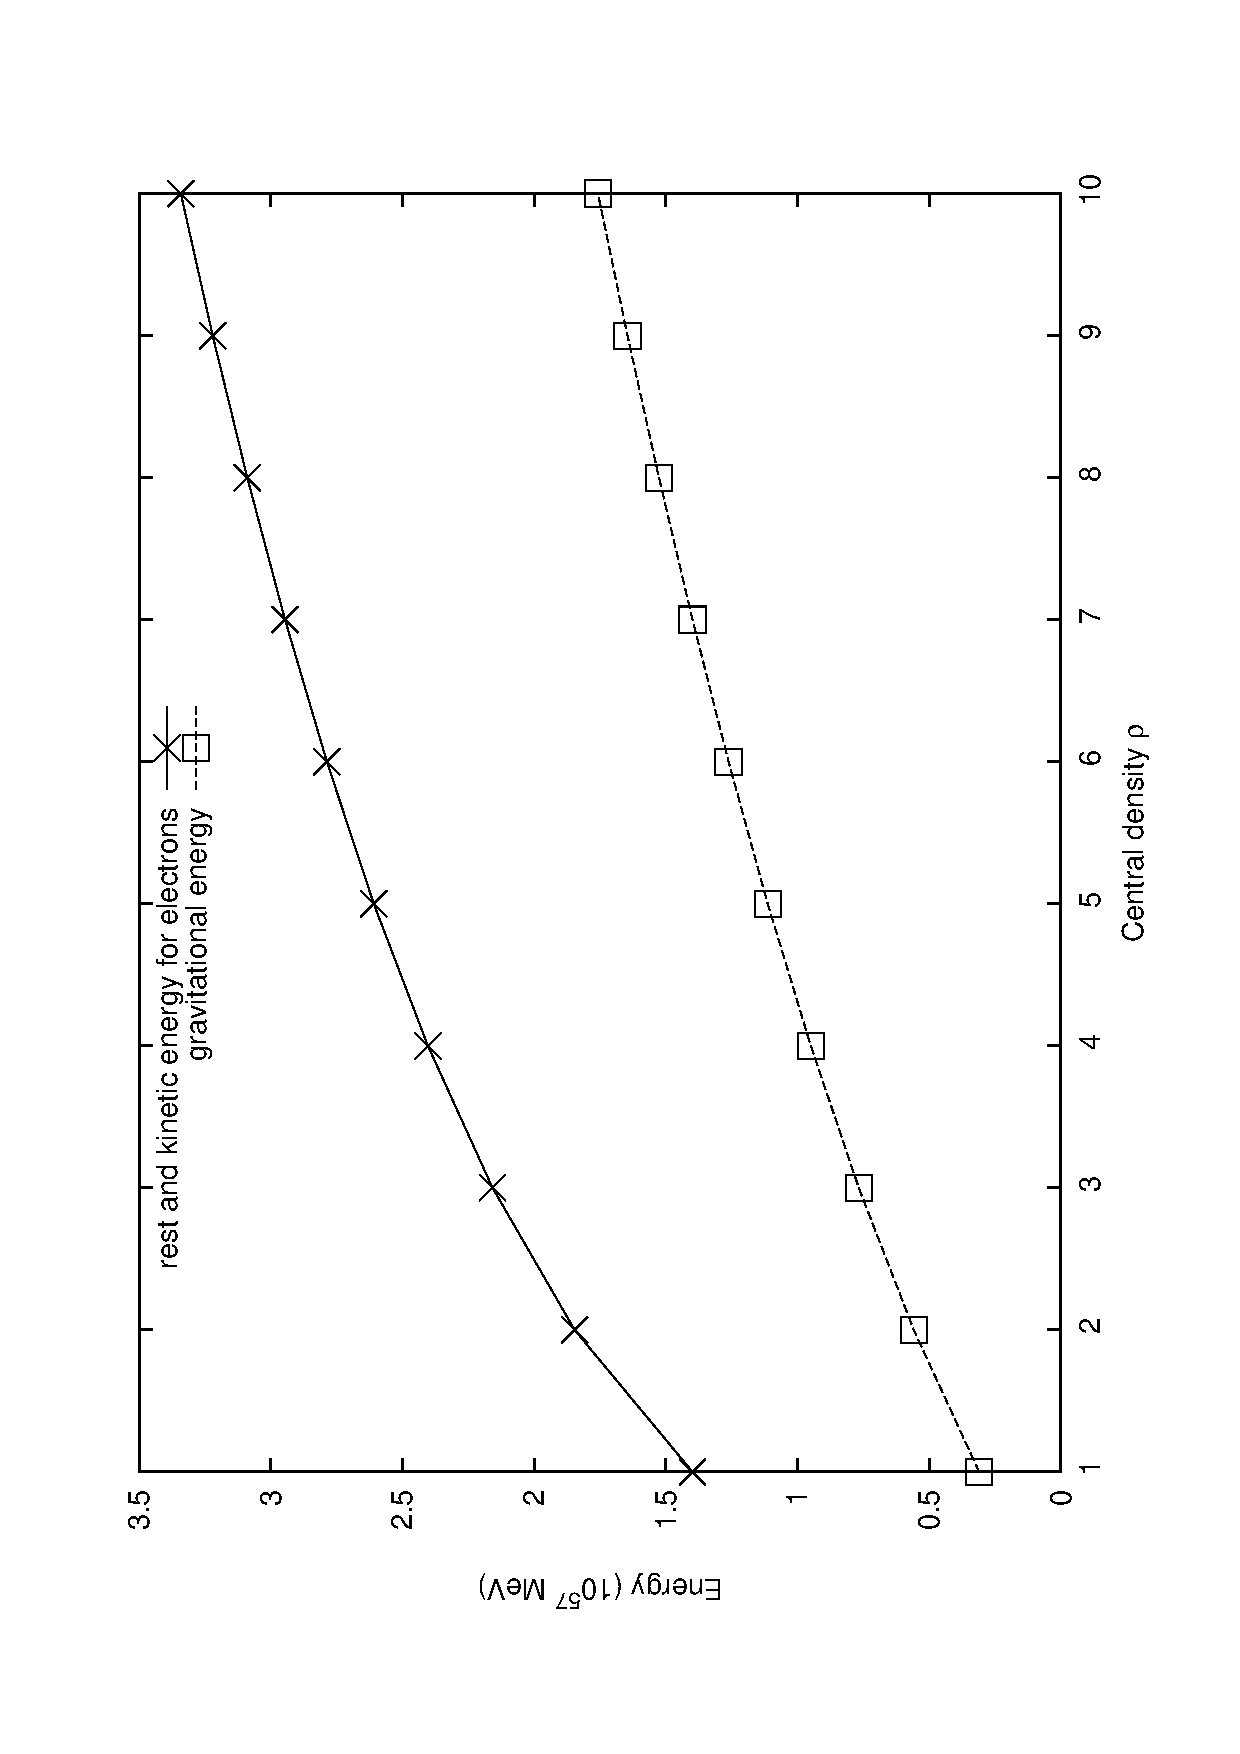
\includegraphics[width=8cm, angle=270]{system_energy}
\caption{Energies for different central densities(note:absolute value is used for the gravitational energy)}
\label{fig:energy}
\end{figure}

\subsection{Comparing with data}
In the previous calculation, we assume $Y_e=1$, which corresponds to planet only containing hydrogen. If we consider other elements as the building block for the planet, we need have different $Y_e$, for example $Y_e^{^{56}\text{Fe}}=0.464,Y_e^{^{12}\text{C}}=0.5$. As $r \propto Y_e$ and $m\propto Y_e^2$, we can just scale the result from table{\ref{tab:rho_dependence}} and get the result for $^{12}$C based planet and $^{56}$Fe based planet, as in table(\ref{tab:Fe},\ref{tab:C}). Masses and radii of the three white dwarf stars Sirius B, 40 Eri B and Stein 2051 have been determined from observations to be ($1.053\pm0.028 M_{\odot}$,$0.0074\pm0.0006R_{\odot}$),($0.48\pm0.02M_{\odot}$,$0.0124\pm0.0005R_{\odot}$) and ($0.72\pm0.08M_{\odot}$,$0.0115\pm0.0012R_{\odot}$).If we compare these data with table(\ref{tab:Fe},\ref{tab:C}), we can find Sirius B fits between central density $\rho=10^1$ and $\rho=10^2$ in table(\ref{tab:C}), which means this planet is built mainly by $^{12}$C. 40 Eri B fits between $\rho=10^0$ and $\rho=10^1$ in table(\ref{tab:Fe}) and Steein 2051 fits between $\rho=10^0$ and $\rho=10^1$ in table(\ref{tab:Fe}) which means these two planets contains mostly $^{56}$Fe, but with different densities.
\begin{table}[H]
\centering
\begin{tabular}{|c|c|c|c|c|}
\hline
$\rho_c /\rho_0$& $10^{-1}$& $10^{0}$ & $10^{1}$  & $10^{2}$  \\
\hline
radius /$R_{\odot}$& 0.0193637&  0.0128736&   0.0082028&  0.0049166\\
\hline
mass /$M_{\odot}$& 0.171653&  0.433736&  0.796242&  1.06463\\
\hline
$\rho_c /\rho_0$&  $10^{3}$  & $10^{4}$  & $10^{5}$  & $10^{6}$ \\
\hline
radius /$R_{\odot}$& 0.00274994& 0.00143917& 0.000715194 & 0.000343931\\
\hline
mass /$M_{\odot}$&1.18567&  1.22477&  1.23499 &  1.23738\\
\hline
\end{tabular}
\caption{Dependence of mass and radius on central density for $^{56}Fe$ based planet}
\label{tab:Fe}
\end{table}

\begin{table}[H]
\centering
\begin{tabular}{|c|c|c|c|c|}
\hline
$\rho_c /\rho_0$& $10^{-1}$& $10^{0}$ & $10^{1}$  & $10^{2}$  \\
\hline
radius /$R_{\odot}$& 0.020866&  0.0138724&   0.00883931&  0.00529806\\
\hline
mass /$M_{\odot}$& 0.199322&  0.503651&  0.92459&  1.23624\\
\hline
$\rho_c /\rho_0$&  $10^{3}$  & $10^{4}$  & $10^{5}$  & $10^{6}$ \\
\hline
radius /$R_{\odot}$& 0.0029633& 0.00155083& 0.000770684 & 0.000370616\\
\hline
mass /$M_{\odot}$&1.37679&  1.42219&  1.43406 &  1.43683\\
\hline
\end{tabular}
\caption{Dependence of mass and radius on central density for $^{12}C$ based planet}
\label{tab:C}
\end{table}

\section{Conclusion}
 In the project, a code based on 4th-order Runge-Kutta method is developed to solve the mechanical equilibrium equation for white dwarf stars. The algorithm is found to be quite stable, with step in the order of $10^2$, we still have the correct result in the fourth digit after the decimal point. Central density is found to be essential to determine size and mass of the dwarf stars. Larger central density leads to smaller size of the planet, but also heavier mass. The total kinetic and rest energy of electrons and gravitational energy of the planet are calculated. They both increase with central density and the ratio between these two energies stays almost the same. The parameter $Y_e$ reflects the nucleus which the white dwarf star mainly built up with. By comparing with our calculation, we believe Sirius B is mainly composed by $^{12}$C. 40 Eri B and Stein 2051 are believed to be mainly composed by $^{56}$Fe




\bibliographystyle{plain}         %obtained from the .bib file
\bibliography{project}


\end{document}